\documentclass[11pt]{article} % use larger type; default would be 10pt

\usepackage{graphicx}
\usepackage{amsmath}
\usepackage{fullpage}
\usepackage[parfill]{parskip}

\title{ME 597 Lab 2 Report}
\author{Iain Peet \and Andrei Danaila \and Ming Ma \and Abdel Hamid \and Ahmed Salam}

\begin{document}
\maketitle

\clearpage

\section{Introduction}

%TODO: complete this.
Placeholder.

\section{Extended Kalman Filter Design}

\subsection{Motion Model}
The robot motion model has the following state:
\begin{equation}
x_t = 
\left[ \begin{array}{c}
v_f \\
\psi \\
x \\
y
\end{array} \right] _t
\end{equation}
Where $v_f$ is forward velocity, $\psi$ is heading, and $x$ and $y$ are position in the horizontal plane.  

The inputs to the system are:
\begin{equation}
u_t =
\left[ \begin{array}{c}
V_m \\
\delta
\end{array} \right] _t
\end{equation}
Where $V_m$ is motor power, and $\delta$ is steering angle.

The following differential equations define $v_f$, $\psi$, $x$, and $y$:
\begin{equation}
\dot{v_f} = -\alpha v_f + K \alpha V_m
\label{vf}
\end{equation}
Where $K$ and $\alpha$ are constants which may be found empirically.
\begin{equation}
\dot{\psi} = \frac{v_f}{L} sin(\delta)
\end{equation}
Where $L$ is wheelbase length,
\begin{equation}
\dot{x} = v_f cos( \psi )
\end{equation}
and
\begin{equation}
\dot{y} = v_f sin( \psi )
\label{y}
\end{equation}

The motion model is therefore:
\begin{equation}
\dot{x_t} = \left[ \begin{array}{c} 
-\alpha v_f + K \alpha V_m \\
\frac{v_f}{L} sin(\delta) \\
v_f cos( \psi ) \\
 sin( \psi )
\end{array} \right] _t + w_t \quad \quad w_t \sim N(0, Q)
\end{equation}


\subsection{Measurement Models}

A simple measurement model where all states are directly measured is used.  Encoder readings are differentiated to yield direct forward velocity measurements.
The local position system yields direct measurements of heading and planar position.  
GPS can be considered to have the same model as the LPS, with heading directly estimated from successive position measurements, so long as the distance travelled between measurements is large relative to position measurement error.

The measurement model is trivially defined as follows:
\begin{equation}
y_t = \left[ \begin{array}{c} v_f \\ \psi \\ x \\ y \end{array} \right]_t + v_t 
\quad \quad v_t \sim N(0,R)
\end{equation}

\subsection{Prediction}

The a priori state expectation is computed from the motion model by
\begin{equation}
\bar{x}_k = f(\hat{x}_{k-1}, u_{k-1})
\end{equation}
Where $f$ may be trivially derived from equations \ref{vf} - \ref{y}. 

The a priori covariance is computed by linearizing about the current state:
\begin{equation}
\bar{P}_k = A_kP_{k-1}A_k^T + W_kQ_{k-1}W_k^T
\end{equation}
Where $A_k$ is the Jacobian, $\frac{\delta f}{\delta x} | _{\hat{x}_{k-1}, u_{k-1}}$:
\renewcommand{\arraystretch}{1.4}
\begin{equation}
\left[ \begin{array}{cccc}
-\alpha T & 0 & 0 & 0 \\
\frac{T}{L} sin( \delta _{k-1} ) & 1 & 0 & 0 \\
T cos(\psi _{k-1}) & - v_{f,k-1} T sin( \psi _{k-1}) & 1 & 0 \\
T sin(\psi _{k-1}) & v_{f,k-1} T cos ( \psi _{k-1}) & 0 & 1 \\
\end{array} \right]
\end{equation}
\renewcommand{\arraystretch}{1}
And $W_k$ is the Jacobian of $x_k$ with respect to process noise, which is simply $I$ in our motion model.

\subsection{Correction}

The a priori state estimate is corrected by sensor measurements.  First, the Kalman gain is computed:
\begin{equation}
K_k = \bar{P}_k H_k^T ( H_k \bar{P}_k H_k^T + V_k R_k V_k^T ) ^{-1}
\end{equation}
Where $H_k$ is the Jacobian of $y_k$ with respect to $x_k$, and $V_k$ is the Jacobian of $y_k$ with respect to measurement noise.   For our measurement model, $H_k$ and $V_k$ are both $I$.

The a posteriori state expectation and covariance can then be computed:
\begin{equation}
\hat{x}_k = \bar{x}_k + K_k (y_k - \bar{x}_k)
\end{equation}
and
\begin{equation}
P_k = (I - K_k H_k) \bar{P}_k
\end{equation}

\subsection{Simulation Results}

\begin{figure}[hbt]
 \centering
 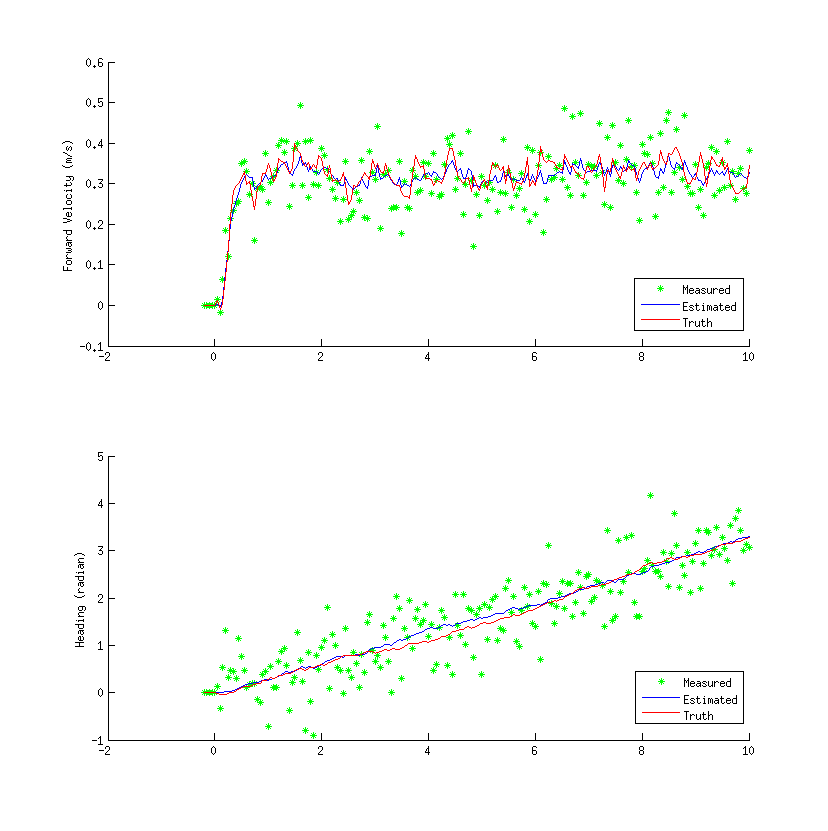
\includegraphics[scale=0.60]{ekf_sim_vh.png}
 \caption{Simulated EKF estimation of forward velocity and heading}
 \label{ekf_s_vh}
\end{figure}

\begin{figure}[hbt]
  \centering
  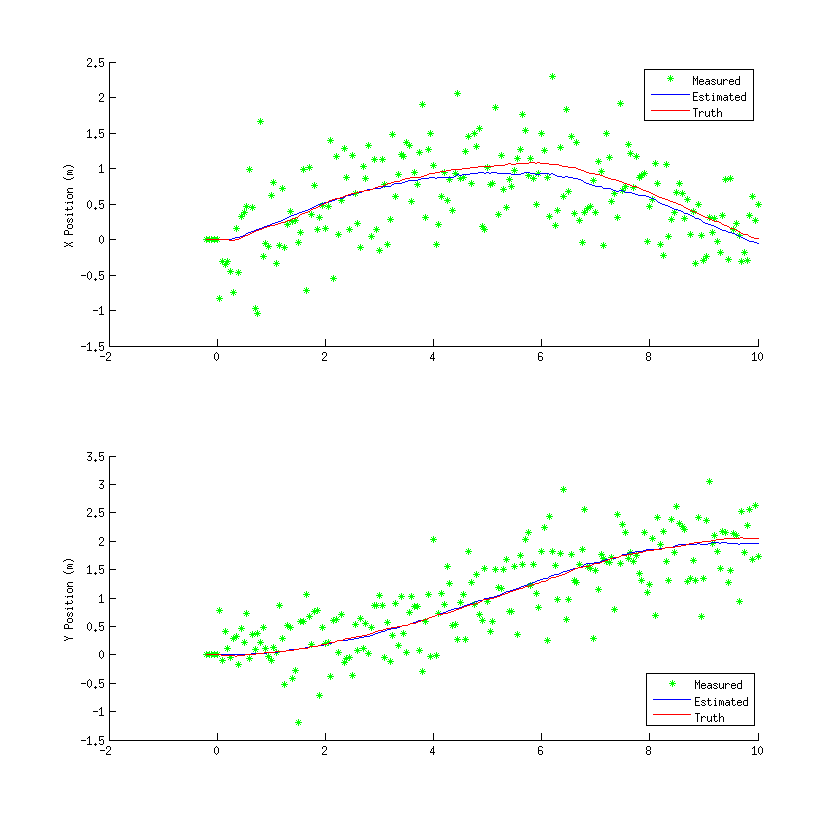
\includegraphics[scale=0.60]{ekf_sim_xy.png}
  \caption{Simulated EKF estimation of planar position}
  \label{ekf_s_xy}
\end{figure}

\clearpage

\subsection{Empirical Results}

\begin{figure} [hbt]
 \centering
 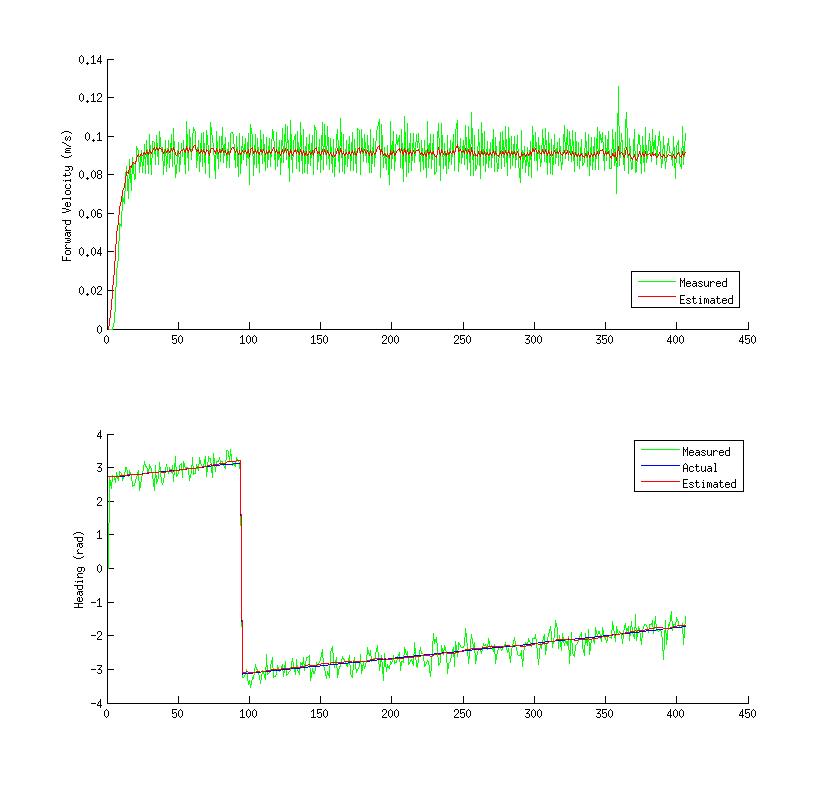
\includegraphics[scale=0.65]{ekf_meas_vh.png} 
 \caption{EKF estimation of forward velocity and heading}
 \label{ekf_m_vh}
\end{figure}

\begin{figure} [hbt]
 \centering
 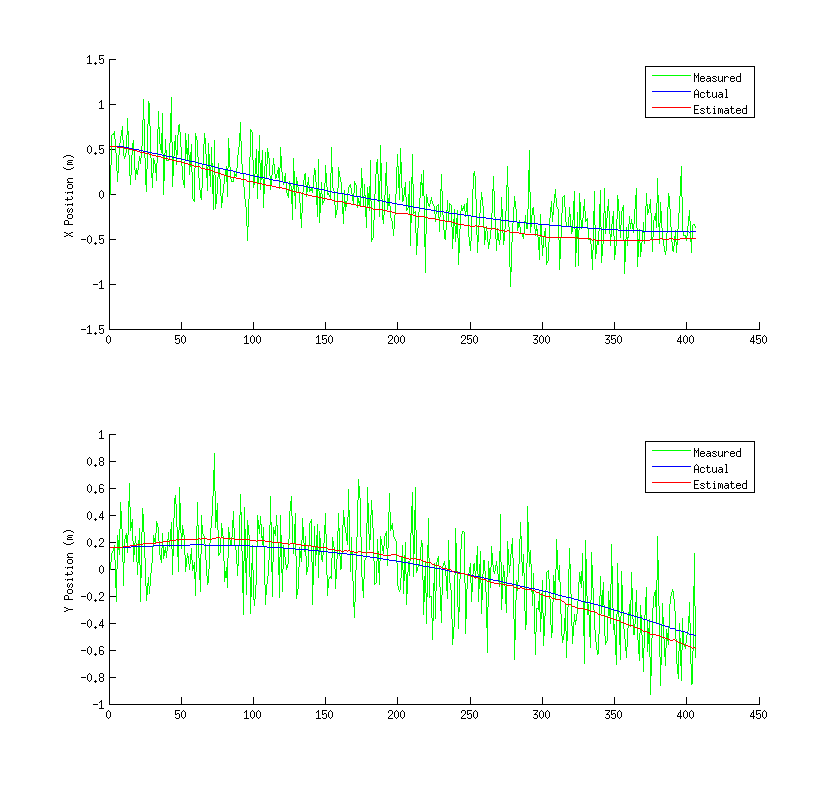
\includegraphics[scale=0.65]{ekf_meas_xy.png}
 \caption{EKF estimation of planar position}
 \label{ekf_m_xy}
\end{figure}

The local positioning system has been found to be extremely accurate.  Practically speaking, the EKF presents little useful gain over the accuracy of the LPS measurements.  We can, however, test the performance of the EKF with less accurate position data, by taking LPS data as ground truth, adding noise to the LPS data, and providing the resulting noisy data to the EKF.

Figures \ref{ekf_m_vh} and \ref{ekf_m_xy} show the estimates produced by the EKF, applied to actual system inputs and noise-corrupted LPS measurements.  It can be seen that the EKF does an excellend job of recovering the original LPS measurement data.  Although we do not have good ground truth measurements for velocity, the velocity estimates do seem reasonable.

\clearpage

\section{Mapping Design}
As it moves, the robot is required use LIDAR data to produce an occupancy grid map of its surroundings.  In addition to EKF state estimates, the mapping algorithm will require an inverse measurement model for the LIDAR.

\section{LIDAR Measurement Model}
The LIDAR provides a sequence of range measurements $r_i$, each of which is made in a different direction, $\phi_i$:

\begin{equation}
r = \{r_1 \dots r_k\} \quad r_i \in [r_{min}, r_{max}]
\end{equation}

\begin{equation}
\phi = \{\phi_1 \dots \phi_k\} \quad \phi_i \in [\phi_{min}, \phi_{max}]
\end{equation}

\section{Inverse LIDAR Measurement Model}
In order to compute an occupancy grid, we must use LIDAR to determine whether or not a particular grid cell is occupied.  For any given cell, there are three possibilities:

\begin{enumerate}
 \item At least one scanline passes through the cell, but no range measurements fall within the cell.
 \item At least one range measurement falls within the cell.
 \item No scanlines pass through the cell.
\end{enumerate}

In the first case, it can be inferred with confidence that the cell is unoccupied.  
In the second case, it is clear that the cell contains an object.  
The third case arises either when a cell is obscured by a nearby object, or when the cell is outside of the area swept by the LIDAR.  In the third case, no information is about the status of the cell.

In order to evaluate the state of a cell, we find the scanline which passes closest to the centre of the cell:

\begin{equation}
i_{nearest} = \underset{i}{\operatorname{argmin}} \quad | \phi_i - tan^{-1}(\frac{y_c - y_r}{x_c - x_r}) |
\end{equation}

Where $(x_c, y_c)$ are the co-ordinates of the centre of the cell, and $(x_r, y_r)$ are the current co-ordinates of the robot.  

Once $i_{nearest}$ is known, the range measurement $r_{i,nearest}$ is compared against the distance to the cell.  If the measured range is within some threshold $\alpha$ of the distance to the cell, it is considered likely that the cell is occupied.  If the range measurement is substantially greater than the distance to the cell, it is considered likely that the cell is unoccupied.  Finally, if the range measurement is less than the distance to the cell, no information is obtained about the state of the cell.

This is an extremely simplistic inverse measurement model.  Uncertainty in the position and heading of the robot are ignored.  Uncertainty in scanline direction is ignored, and the arc covered by a particular range measurement is assumed to be equal to the angular separation of consecutive measurements.  The use of the scanline which passes nearest the centre of the cell ignores the possibility that multiple scanlines might pass through a single cell, or, alternatively, that even the nearest scanline does not pass through the cell at all.  

\subsection{Simulation Results}

% TODO: matlab simulation.  
Placeholder.

\subsection{Empirical Results}

% TODO: requires LPS.
Placeholder.

\section{Conclusions}

% TODO: need a whole raft of results.
Placeholder.

\end{document}